\chapter{Motion-Aware Unitを用いた1波長を入力とした紫外線像の全球時系列予測}
  \section{実験概要}
  この実験では入力、出力ともに211Åフィルターで得られたデータを利用した。
  これは 211Åフィルターで撮影された紫外線像が、コロナホールと活動領域といった、二つの太陽円盤上の大規模構造をバランスよく明瞭に表現し、本研究のモデルの効果検証に適していると考えたためである。
  モデルにはMotion-Aware Unitを用い、1波長のデータを入力として、全球の時系列予測を行った。
  この実験の概要を図\ref{fig:exp1_overview}にて視覚的に表現する。

  \begin{figure}[htpb]
    \centering
    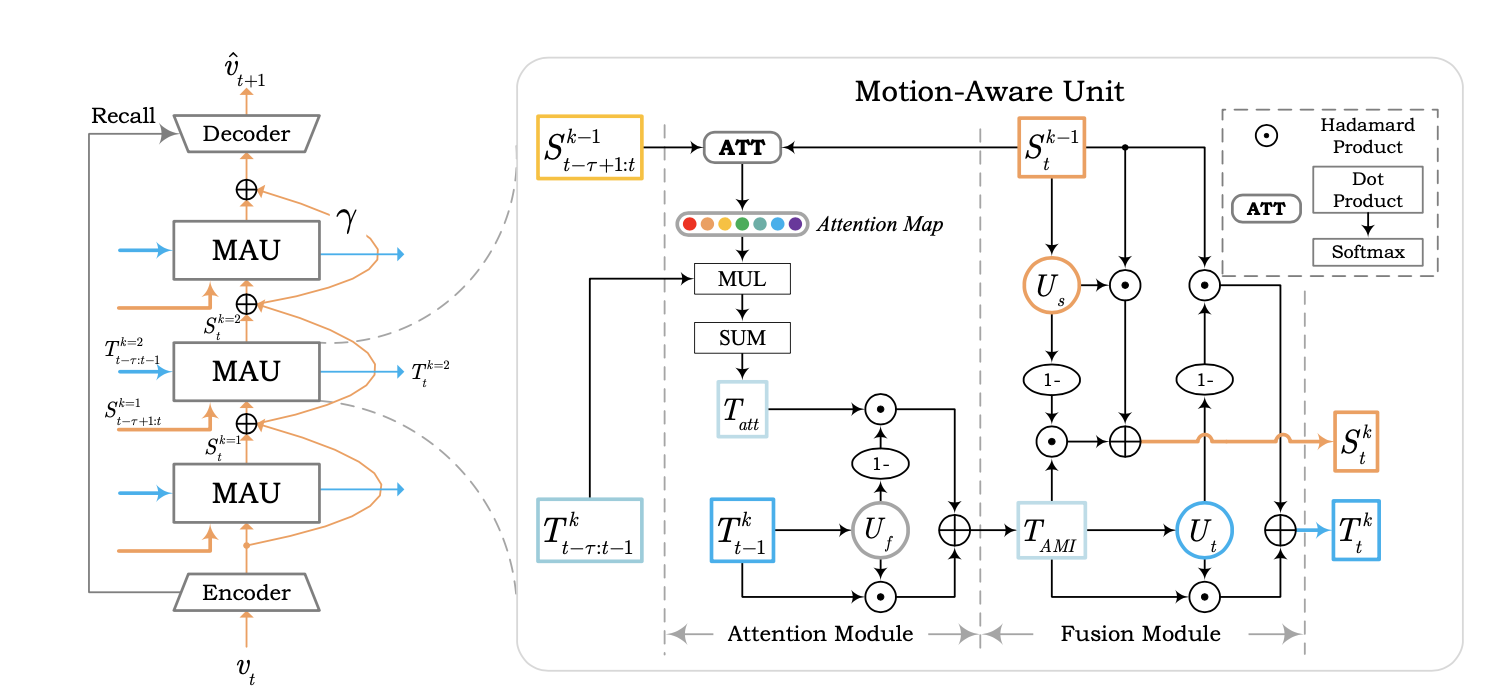
\includegraphics[width=\textwidth]{figures/mau.png}
    \caption{実験の概念図。モデルにはMotion-Aware Unitを用い、1波長のデータを入力として、全球の時系列予測を行った。}
    \label{fig:exp1_overview}
  \end{figure}

  \section{実験設定}
    各ハイパーパラメータの設定を表\ref{tab:exp1_hyperparameters}に示す。バッチサイズは実験的に決定し、最も安定的に最終的に良好な精度を達成できた値を採用した。また、エポック数は100とした。学習率は0.0005とした。MAU Cell数は、Chang et al. (2019) \cite{chang2021mau} の実験設定を参考に、16とした。
    \begin{table}[htpb]
      \centering
      \begin{tabular}{lc}
      \hline
      ハイパーパラメータ & 値 \\
      \hline\hline
      バッチサイズ & 4 \\
      \hline
      エポック数 & 100 \\
      \hline
      学習率 & 0.0005 \\
      \hline
      損失関数 & MSE \\
      \hline
      チャンネル & 1 \\
      \hline
      カーネルサイズ & (5, 5) \\
      \hline
      MAU Cell数 & 16 \\
      \hline
      \end{tabular}
      \caption{本実験でのハイパーパラメータ設定}
      \label{tab:exp1_hyperparameters}
    \end{table}

  \section{学習の推移}
  学習は図\ref{fig:exp1_learn_progress}のように推移した。学習の初期段階では、学習データに対する損失関数の値が急激に減少しているが、学習が進むにつれて収束に向かって緩やかに減少していることがわかる。
  また、学習損失、検証損失ともに、安定的に減少していることがわかる。
  学習にはNVIDIA RTX A6000を用い、完了までに約14時間を要した。
  \begin{figure}[htpb]
    \centering
    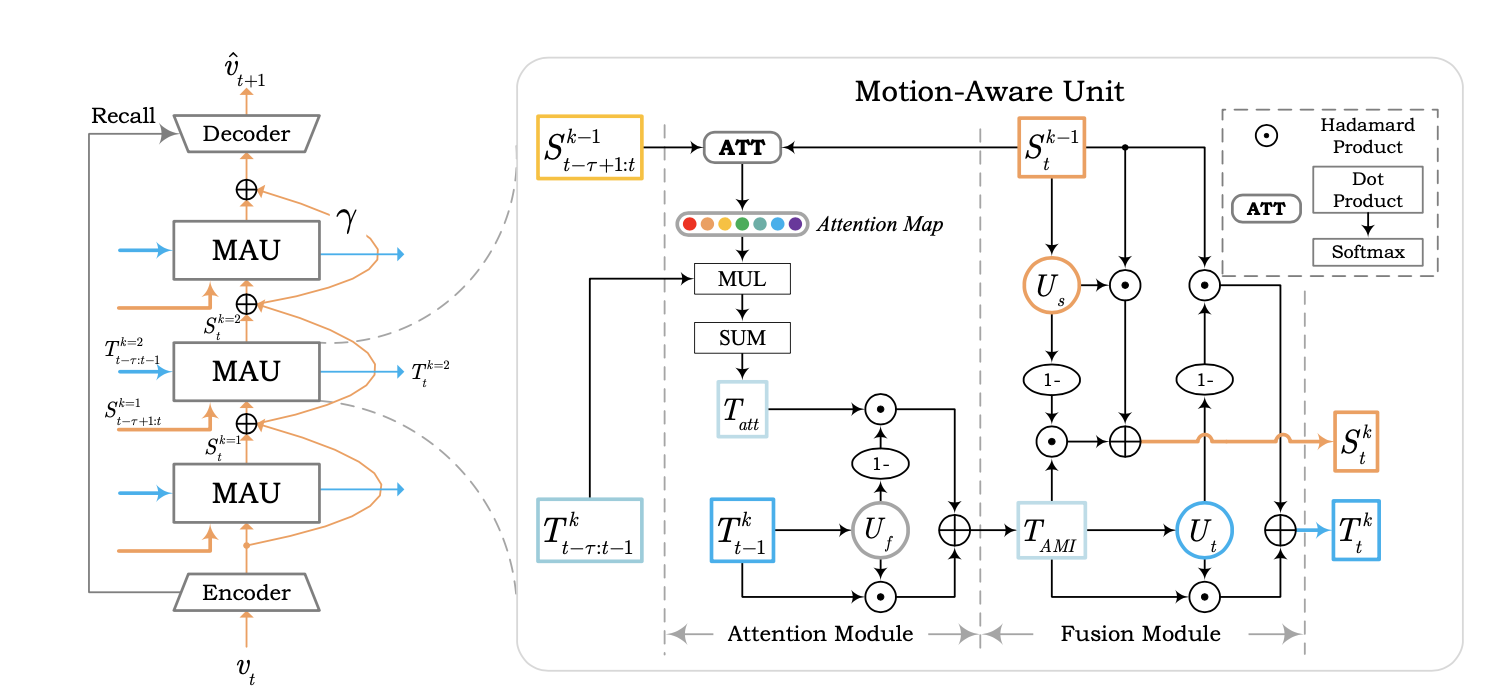
\includegraphics[width=\textwidth]{figures/mau.png}
    \caption{本実験での、学習データ、検証データでの損失関数の推移。どちらも安定的に減少している。}
    \label{fig:exp1_learn_progress}
  \end{figure}

  \section{実験結果}
    図\ref{fig:exp1_gt}および図\ref{fig:exp1_pd}に、この実験での出力例を示す。
    これは学習データに含まれない期間のテストデータである。
    \begin{figure}[htpb]
      \centering
      \vspace*{-2cm} % 上の余白を調整
      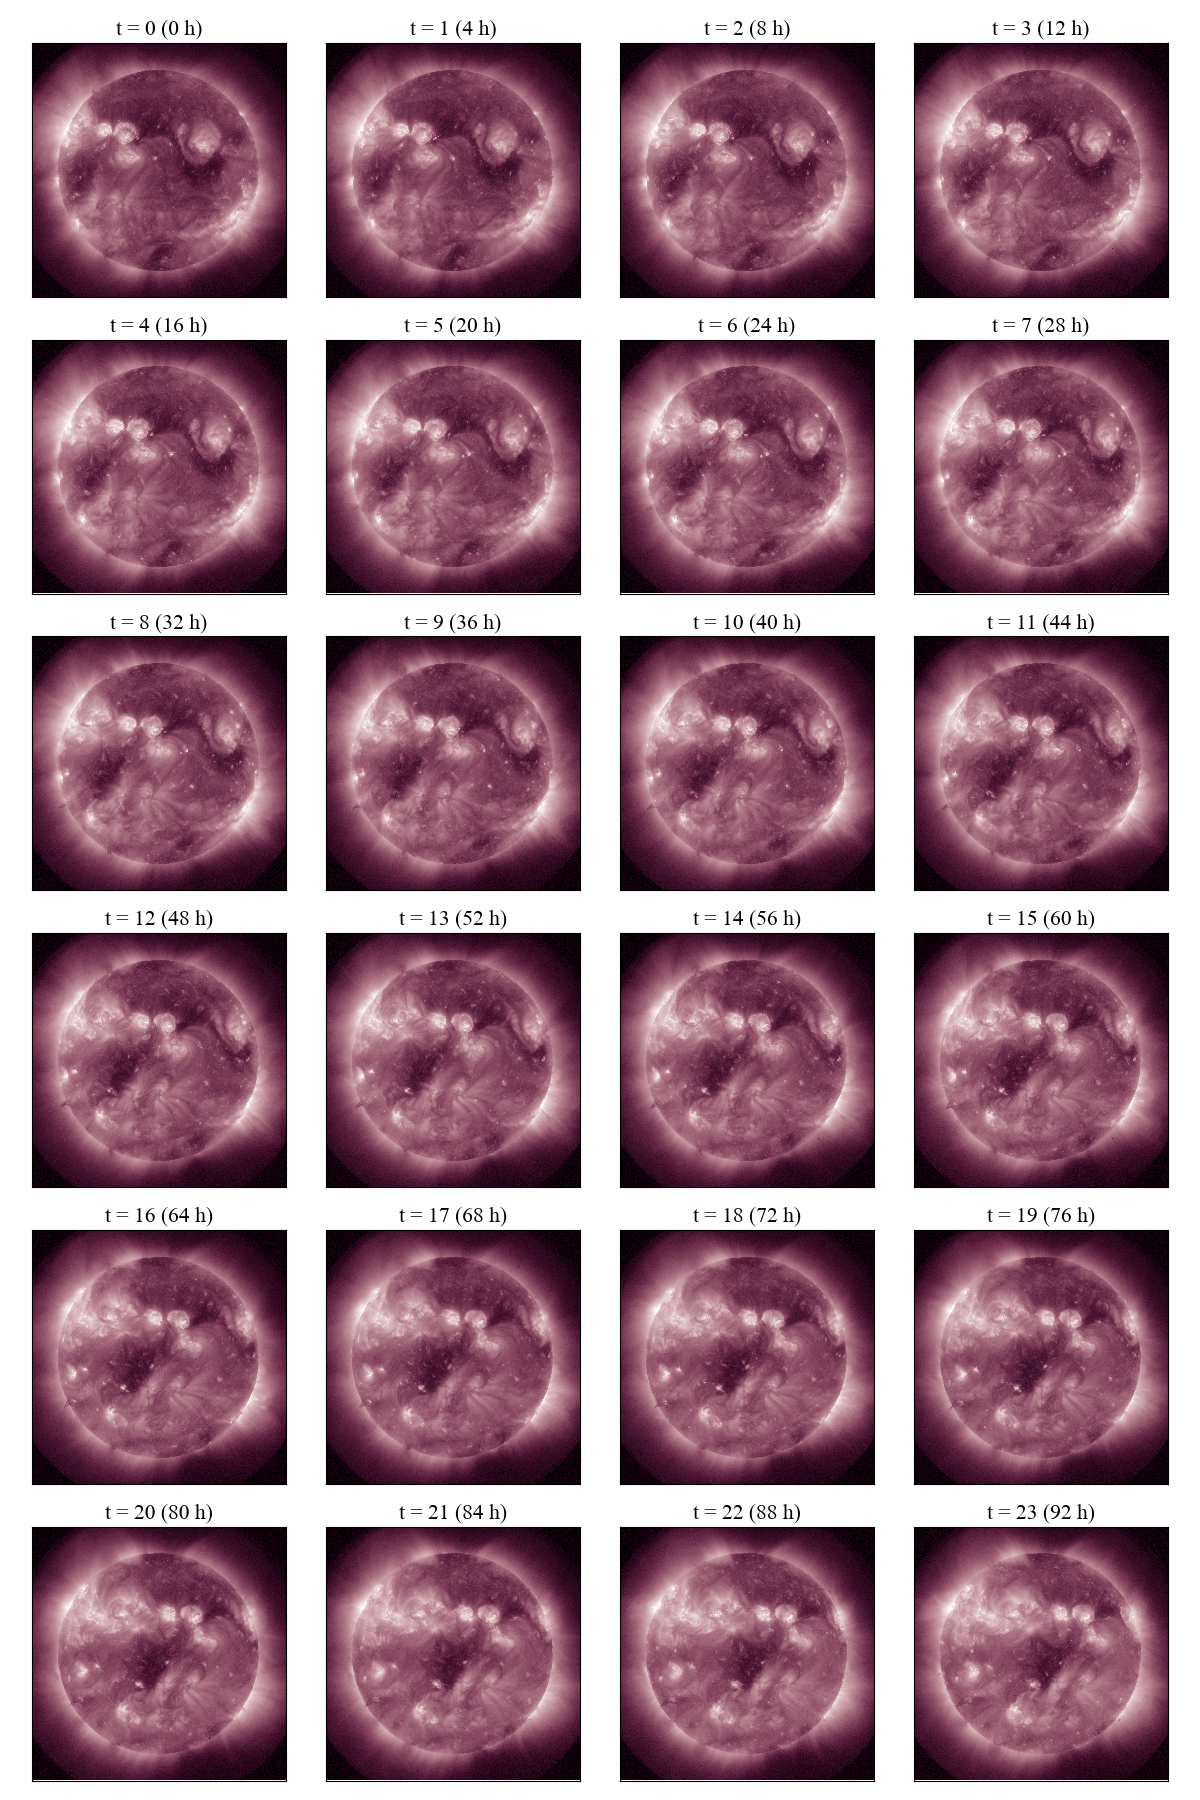
\includegraphics[width=0.95\textwidth]{figures/exp1/gt.png}
      \caption{実際の観測画像の例。2022年2月18日0時から2022年2月22日20時の期間から4時間毎にサンプリングされている。このt=0からt=11までをモデルに入力データとして渡している。モデルはその入力データを元に、t=12からt=23の12枚の画像を予測する。t=12以降の実際の観測画像はモデルに渡されない。}
      \vspace{-1cm} % 下の余白を調整
      \label{fig:exp1_gt}
    \end{figure}
    \begin{figure}[htpb]
      \centering
      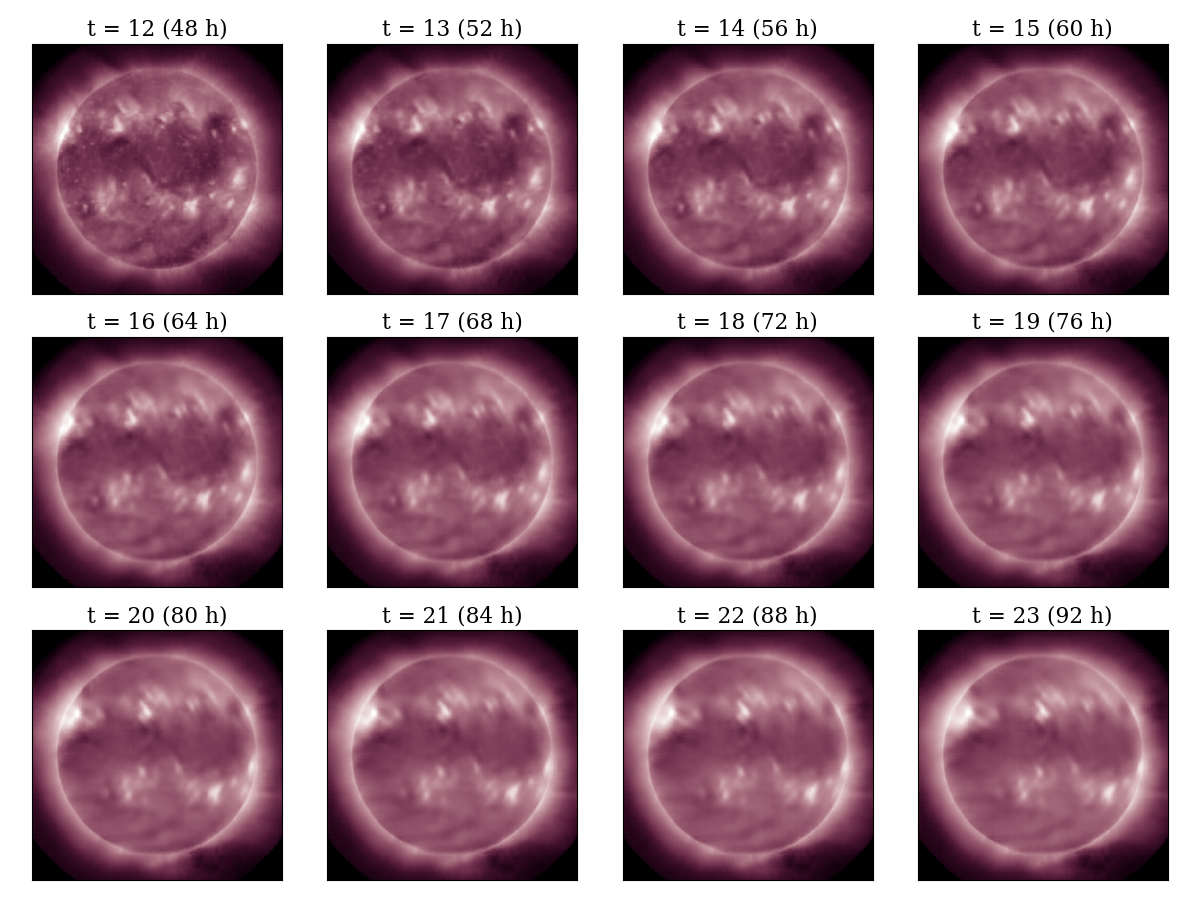
\includegraphics[width=0.95\textwidth]{figures/exp1/pd.png}
      \caption{MAUによる予測画像。対応するタイムステップtの観測画像(図\ref{fig:exp1_gt})と比較することでモデルの再現度を視覚的に評価することができる。大規模な構造は概ね実際の観測画像と合致している。モデルの特性により、時間経過とともに少しずつ予測が不安定になり、ぼやけた見た目になる。}
      \label{fig:exp1_pd}
    \end{figure}
    モデルの出力は、視覚的には実際の観測画像と概ね合致しており、特に自転による大規模構造の移動といった顕著な時間的特徴は再現できていることがわかる。

    動画予測の精度を評価するために、太陽の輝度強度の再現性を定量的、またまたは視覚的に評価する。
    これは、Nishizuka et al. (2018) \cite{nishizuka2018deep} や〜〜〜などの、太陽画像から太陽イベントを予測する先行研究では、その画像中の輝度強度を主要な特徴量として採用していることに基づく。
    この輝度強度の再現性の評価を、さまざまな条件下で行った。はじめに全球での評価を行い、次に経度依存性の評価を行った。最後に、東側リムから出現する活動領域に対する視覚的評価を行った。

    \subsection{全球での評価}
      はじめに全球での評価を行った。
      この評価では、まず輝度強度の平均値と実際の平均値との誤差、構造的類似度(Structual Similarity, SSIM)を計算した。さらに単純差動回転モデルとの比較も行った。
      また、これらの値の時間経過に対する変化を観察し、より不確定性の高い将来の予測に対しても動画予測モデルが有効であるかを検証した。
      
      \subsubsection{平均輝度の再現}
        テストセット全体における、ある時間ステップtの平均輝度の絶対誤差を以下のように計算した。
        \begin{align}
          \bar{E}_{t} & = \frac{1}{N} \sum_{i=1}^{50} | \bar{I}_{\text{Prediction}_{i,t}} - \bar{I}_{\text{Actual}_{i,t}} |
        \end{align}
        ここで、iはテストセットのインデックスを表す。また、\( \bar{I}_{\text{Prediction}_{i,t}} \)は、テストセットi、時間ステップtにおける、モデルから生成された画像から計算された平均輝度を表し、\( \bar{I}_{\text{Actual}_{i,t}} \)は、実際の画像から計算された平均輝度を表す。
        平均輝度は全球(画像中の太陽の球面)に対してのみ行い、画像中の背景や外縁部からはみ出すコロナなどはその計算に含まれない。
        背景から全球に対して切り出される部分は、図\ref{fig:exp1_fulldisk_crop}に示されている。
        この全球の定義および計算は、取得したFITSファイルのヘッダーに記載される太陽の中心および半径に基づいている。
        \begin{figure}[htpb]
          \centering
          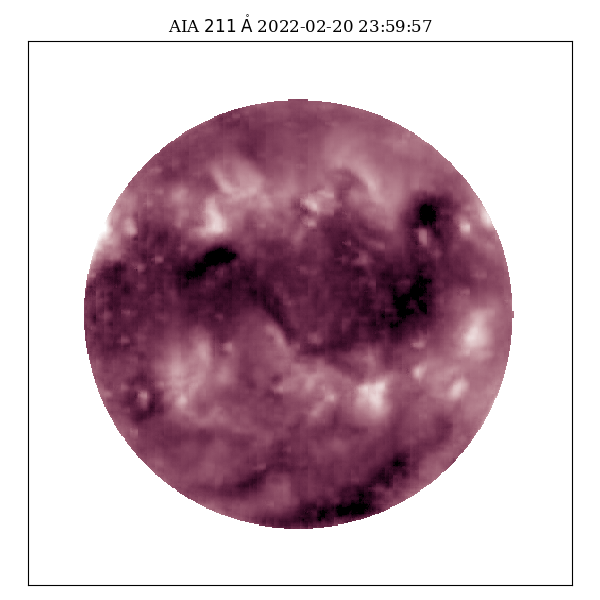
\includegraphics[width=0.7\textwidth]{figures/exp1/crop_map.png}
          \caption{生成した画像から全球部分のみ切り出した画像の例。この部分にのみ平均輝度を計算する。}
          \label{fig:exp1_fulldisk_crop}
        \end{figure}

        モデルの出力の全球での平均輝度と、実際の観測画像との誤差の推移を図\ref{fig:exp1_mean_intensity_line}に示す。
        これは、50のテストセットに対して、各テストセットに含まれる各画像の全球での平均輝度を計算し、その時間ステップごとの平均値を取ったものである。
        \begin{figure}[htpb]
          \centering
          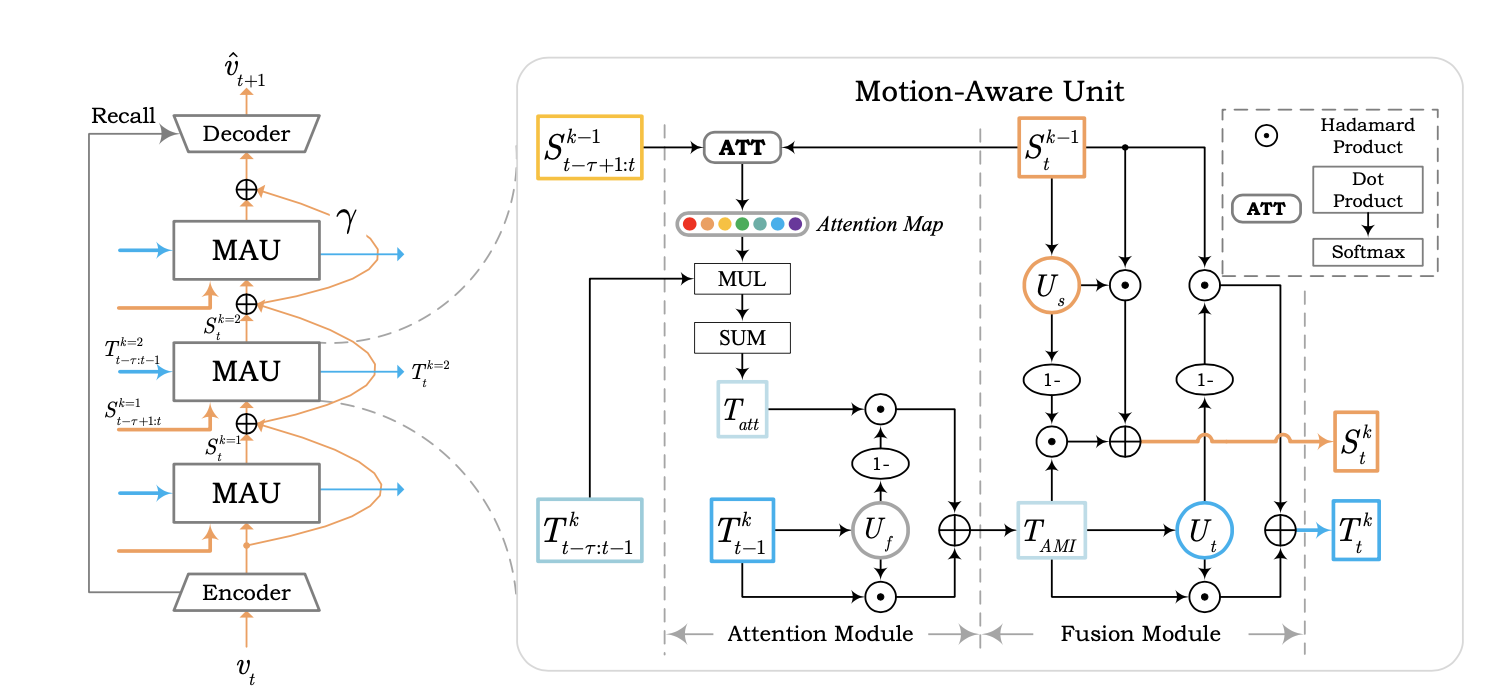
\includegraphics[width=\textwidth]{figures/mau.png}
          \caption{}
          \label{fig:exp1_mean_intensity_line}
        \end{figure}
        
        さらに、入力シークエンスの最後から48時間後の画像の全球での平均輝度と、実際の観測画像との差異を観察する。その散布図\ref{fig:exp1_mean_intensity_scatter}に示す。
        このタイムステップは、出力の最後のタイムステップであり、最も不確定性の高い予測である。
        \begin{figure}[htpb]
          \centering
          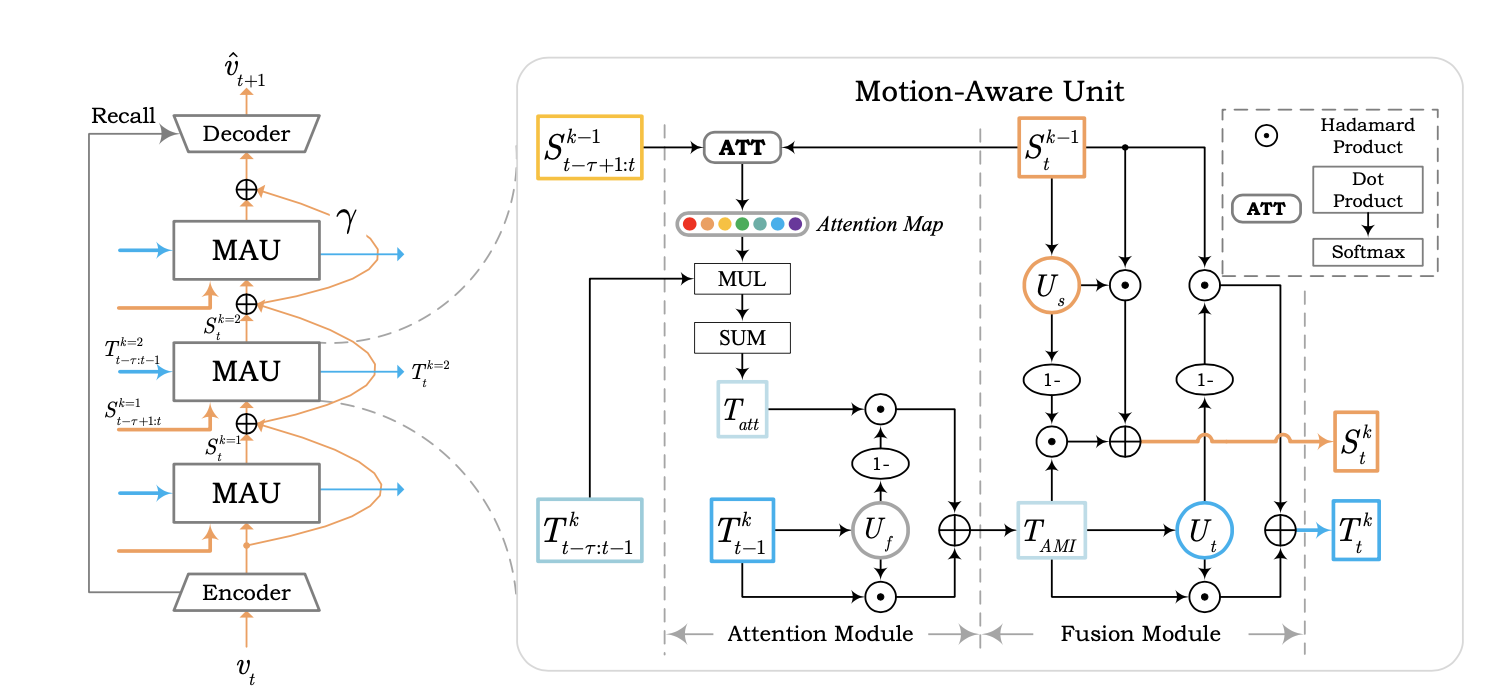
\includegraphics[width=\textwidth]{figures/mau.png}
          \caption{}
          \label{fig:exp1_mean_intensity_scatter}
        \end{figure}

      \subsubsection{画像類似度}
        画像内での構造的再現度とその時間的変化を評価するために、モデルの出力と対応する時間ステップの実際の観測画像の間のSSIMを計算した。
        SSIMは、画像の品質評価を目的として、Wang et al. ( 2004 )\cite{wang2004image}で提案された。
        SSIMは特に構造情報が重要とされる医療画像や衛星画像のような分野で広く使用されている。従来の平均二乗誤差(MSE)やピーク信号対雑音比(PSNR)と比較して、SSIMは人間の視覚システムにより近い知覚品質を提供する。
        従来の手法とは異なり、SSIMは画像の輝度、コントラスト、構造の三つの比較を基にしている。
        SSIMの定義は以下の通りである:
        \begin{equation}
          SSIM(x, y) = \frac{(2\mu_x \mu_y + C_1)(2\sigma_{xy} + C_2)}{(\mu_x^2 + \mu_y^2 + C_1)(\sigma_x^2 + \sigma_y^2 + C_2)},     
        \end{equation}
        ここで、$x$と$y$は比較される二つの画像、$\mu_x$、$\mu_y$はそれぞれの画像の平均輝度、$\sigma_x^2$、$\sigma_y^2$はそれぞれの分散、$\sigma_{xy}$は共分散である。$C_1$と$C_2$は安定性のための小さな定数である。
        
        テストセット全体における、ある時間ステップtのSSIMの平均を以下のように計算した。
        \begin{align}
          \bar{SSIM}_{t} & = \frac{1}{N} \sum_{i=1}^{50} \text{SSIM}_{i,t}
        \end{align}

        SSIMの推移を図\ref{fig:exp1_ssim_line}に示す。画像類似度は、全球での平均輝度と同様に、全球に対してのみ行い、画像中の背景や外縁部からはみ出すコロナなどはその計算に含まれない。

        \begin{figure}[htpb]
          \centering
          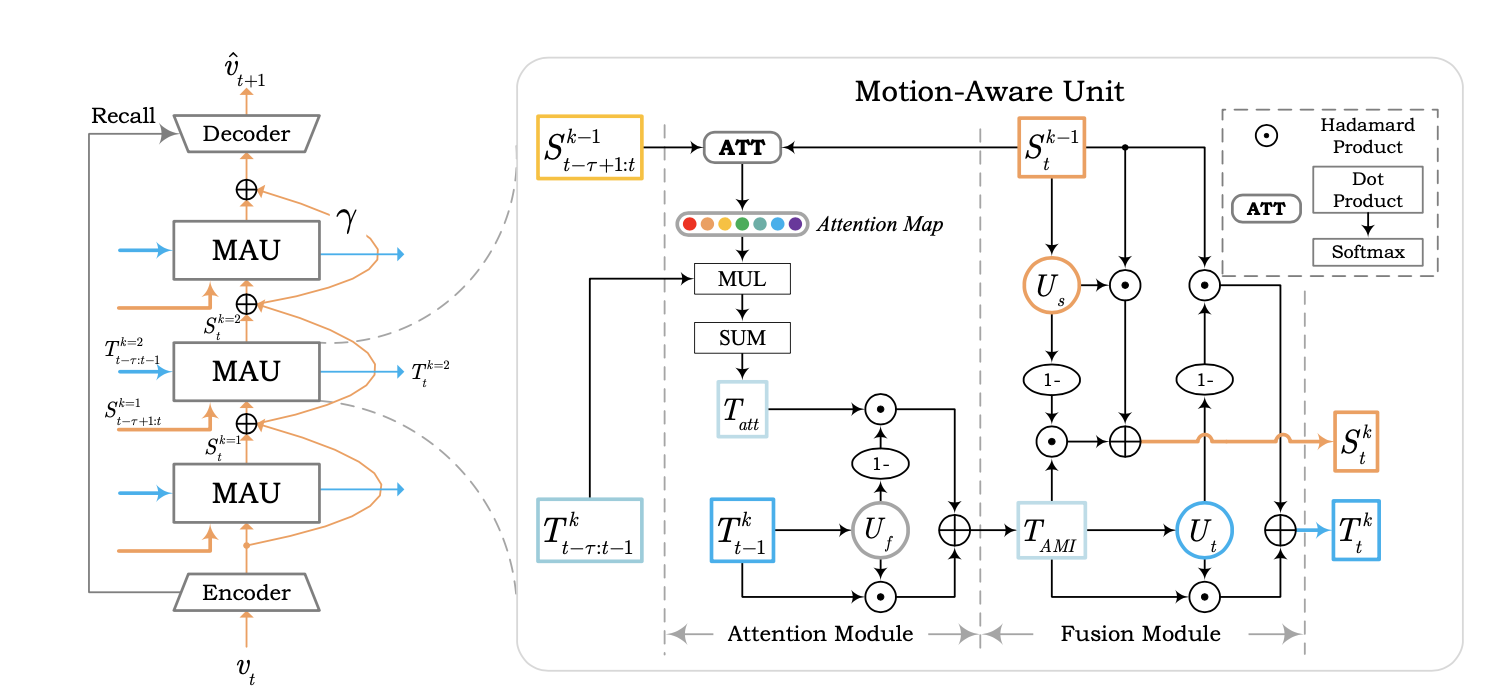
\includegraphics[width=\textwidth]{figures/mau.png}
          \caption{}
          \label{fig:exp1_ssim_line}
        \end{figure}
        
      \subsubsection{単純差動回転モデルとの比較}
        モデルの予測性能をさらに詳細に評価するために、シンプルな差動回転モデルとの比較を行った。
        目視や、平均輝度、SSIMの推移から、モデルの出力は実際の観測画像と概ね合致しており、特に自転による構造的変化などの主要な時間的特徴を再現できていることがわかった。
        ここでは、単純差動回転シミュレーションモデルによる出力と、我々のモデルの出力の再現精度の比較を行った。
        これにより、モデルが単に自転を予測しているのではなく、より複雑な時間的変化を予測できているかを検証した。

        太陽は自転するが、その実体は流体であるため、緯度によって自転速度が異なる。極付近の自転周期は約35日であるが、赤道付近では約25日である。この現象を差動回転と呼ぶ。
        差動回転をシミュレーションする研究は盛んに行われているが、ここでは回転速度を緯度依存としてモデル化するHoward et al. (1990) \cite{howard1990solar}の差動回転モデルを用いた。
        このモデルは、Heliographic緯度\(\theta\)に対する回転速度\(\omega(\theta)\)を以下のように定義する:
        
        \begin{align}
          \omega(\theta) &= A + B \sin^{2}(\theta) + C \sin^{4}(\theta) \\
          \text{where} \quad A &= 2.894 \, \mu\text{rad/s}, \\
          B &= -0.428 \, \mu\text{rad/s}, \\
          C &= -0.370 \, \mu\text{rad/s}
        \end{align}
        このモデルはSunpyに実装されており、\textit{physics.differential\_rotation}というモジュールとして提供されている。
        このモジュールによる画像の生成は、全球の各ピクセルに対して、そのピクセルの緯度に対する回転速度を計算し、その速度で西に向かって各ピクセルを移動させることで行われる。
        この単純差動回転モデルによるシミュレーションの例を図\ref{fig:exp1_sdr_example}に示す。
        比較は、単純差動回転モデルによるシミュレーションと、実際の観測画像との間の平均輝度の絶対誤差を計算し、それを前述の動画予測によるものと比較することで行った。
        この誤差の推移を図\ref{fig:exp1_sdr_line}に示す。
        \begin{figure}[htpb]
          \centering
          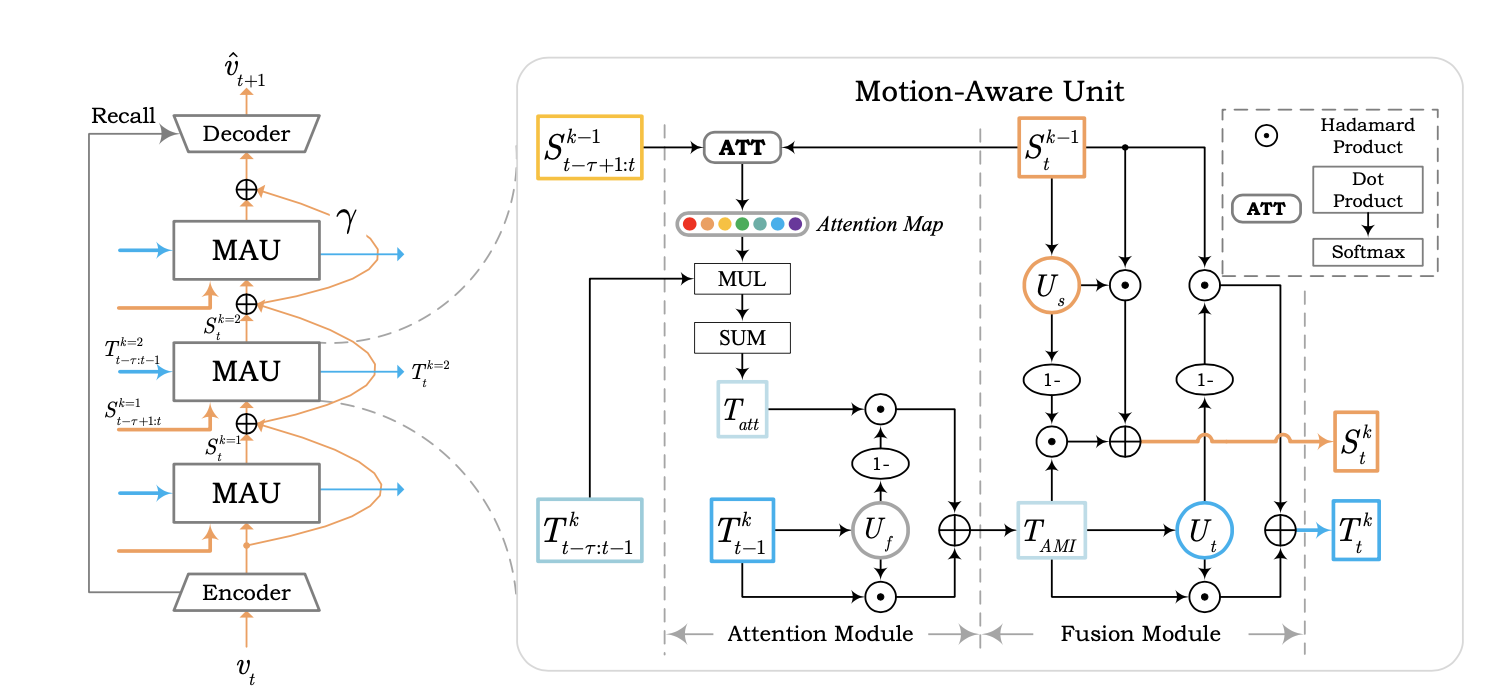
\includegraphics[width=\textwidth]{figures/mau.png}
          \caption{}
          \label{fig:exp1_sdr_example}
        \end{figure}

        \begin{figure}[htpb]
          \centering
          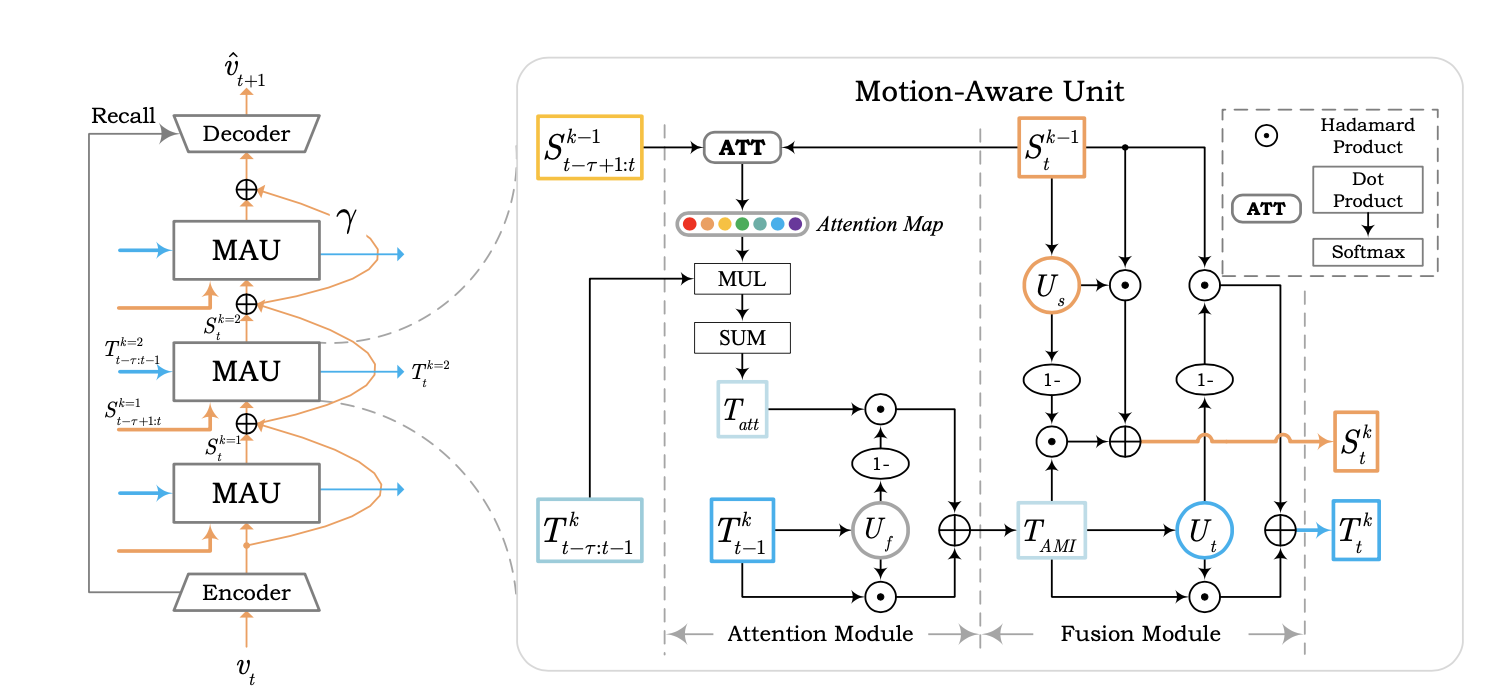
\includegraphics[width=\textwidth]{figures/mau.png}
          \caption{}
          \label{fig:exp1_sdr_line}
        \end{figure}
        
        さらに、出力シークエンスの最後のタイムステップにおいて、単純差動回転モデルによるシミュレーションと、実際の観測画像との差異を観察し、動画予測モデルによる出力と比較した。
        その散布図\ref{fig:exp1_sdr_scatter}に示す。
        
        \begin{figure}[htpb]
          \centering
          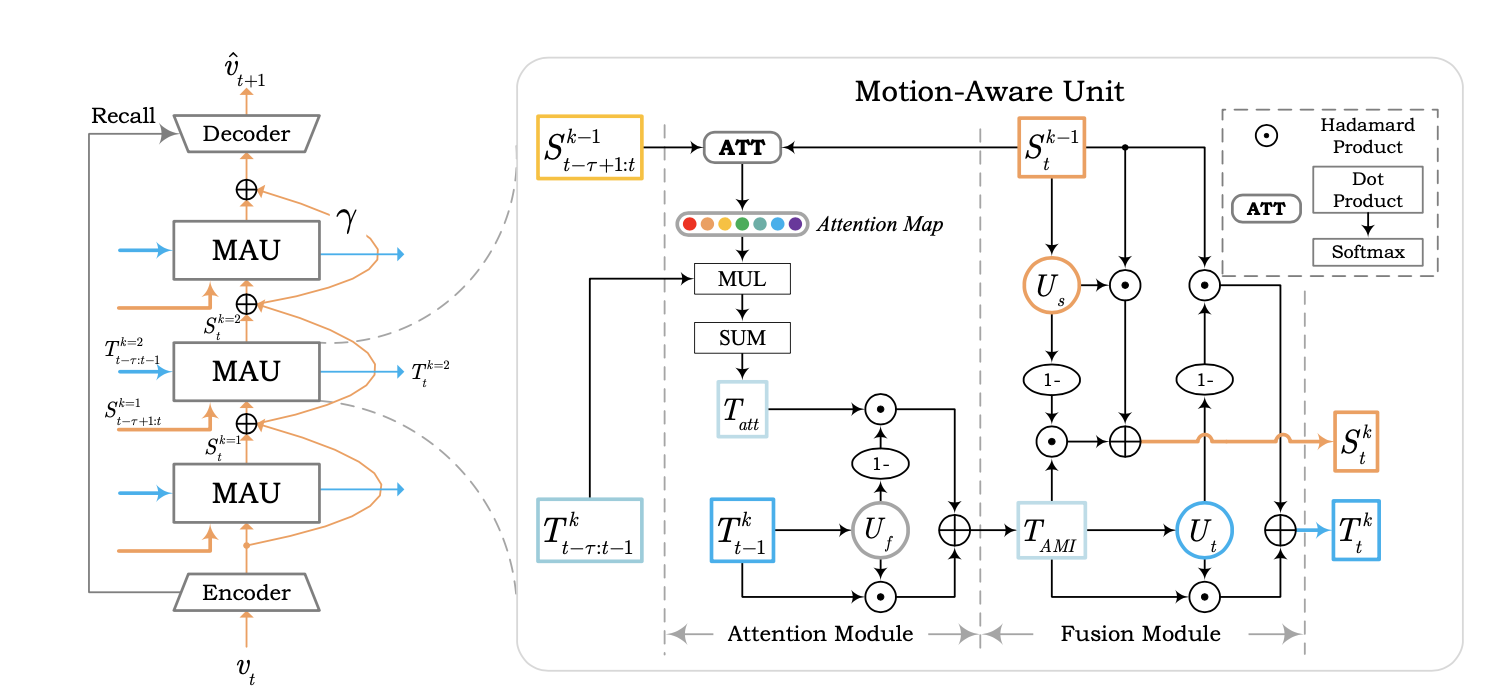
\includegraphics[width=\textwidth]{figures/mau.png}
          \caption{}
          \label{fig:exp1_sdr_scatter}
        \end{figure}
        

    \subsection{経度依存性の評価}
        さらに、予測性能が経度ごとにばらつきがあるかを確認するために、経度ごと予測の再現度を評価した。
        具体的には、Heliographic 座標系における経度-90°から90°までの半球を、36°ごとに5つのセクターに分割した。
        分割の概念図を図\ref{fig:exp1_longitude_division}に示す。
        評価指標には、平均輝度の誤差と、その単純差動回転モデルとの比較を用いた。
        
        \begin{figure}[htpb]
          \centering
          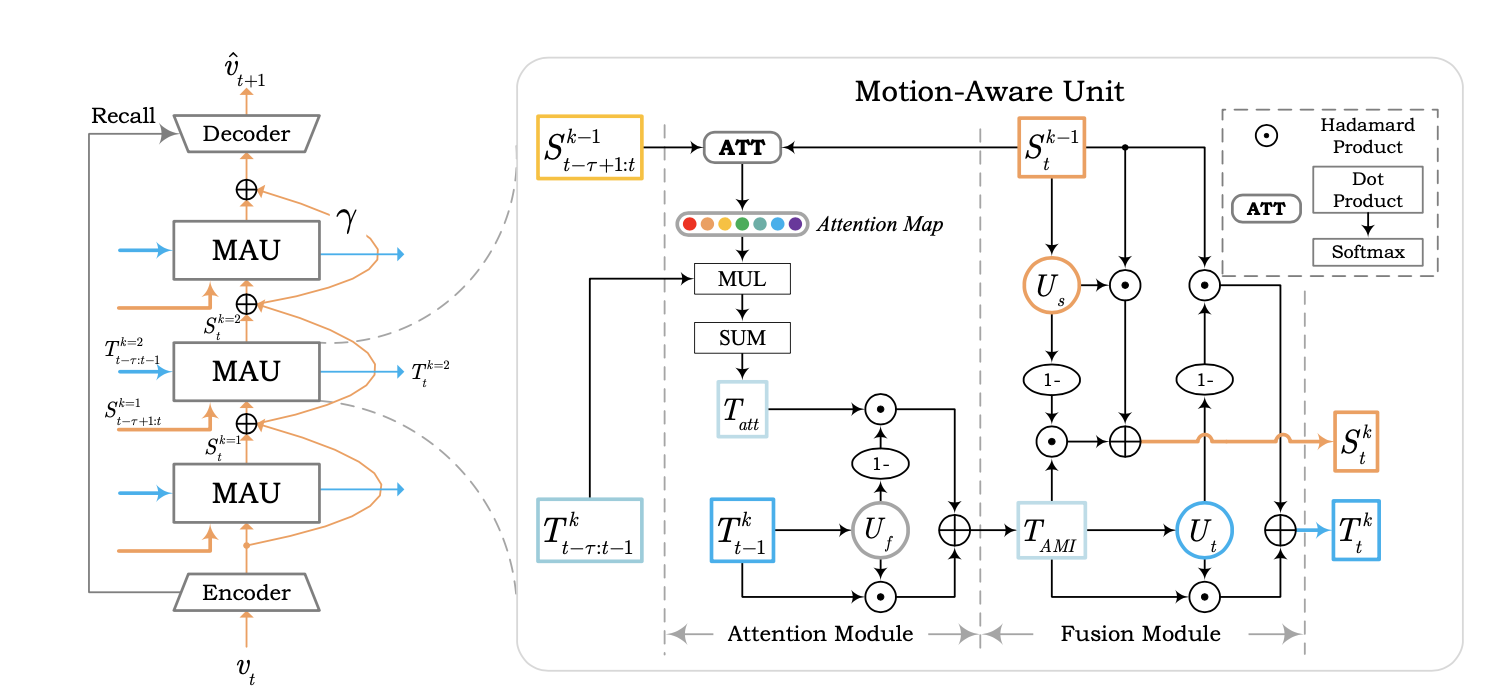
\includegraphics[width=\textwidth]{figures/mau.png}
          \caption{}
          \label{fig:exp1_longitude_division}
        \end{figure}

        \subsubsection{平均輝度とその誤差}
          ここでは、全てのテストセットで各セクターごとの平均輝度を計算し、対応する時間ステップの実際の観測画像との間の絶対誤差を計算した。
          ここで、ある時間ステップt、ある経度セクターlにおける平均輝度の絶対誤差\( \bar{E}_{l,t} \)は以下のように定義される:
          
          \begin{align}
            \bar{E}_{l, t} & = \frac{1}{N} \sum_{i=1}^{50} | \bar{I}_{\text{Prediction}_ {i, l, t}} - \bar{I}_{\text{Actual}_{i, l, t}} | \\
          \end{align}
            
          ここで、iはテストセットのインデックスを表す。また、\( \bar{I}_{\text{Prediction}_{i, l, t}} \)は、テストセットi、時間ステップt、経度セクターlにおける予測された平均輝度を表し、\( \bar{I}_{\text{Actual}_{i, l, t}} \)は、実際の平均輝度を表す。  

          このように計算された誤差率の時間推移を図\ref{fig:exp1_mean_intensity_longitude_line}に示す。
          
          \begin{figure}[htpb]
            \centering
            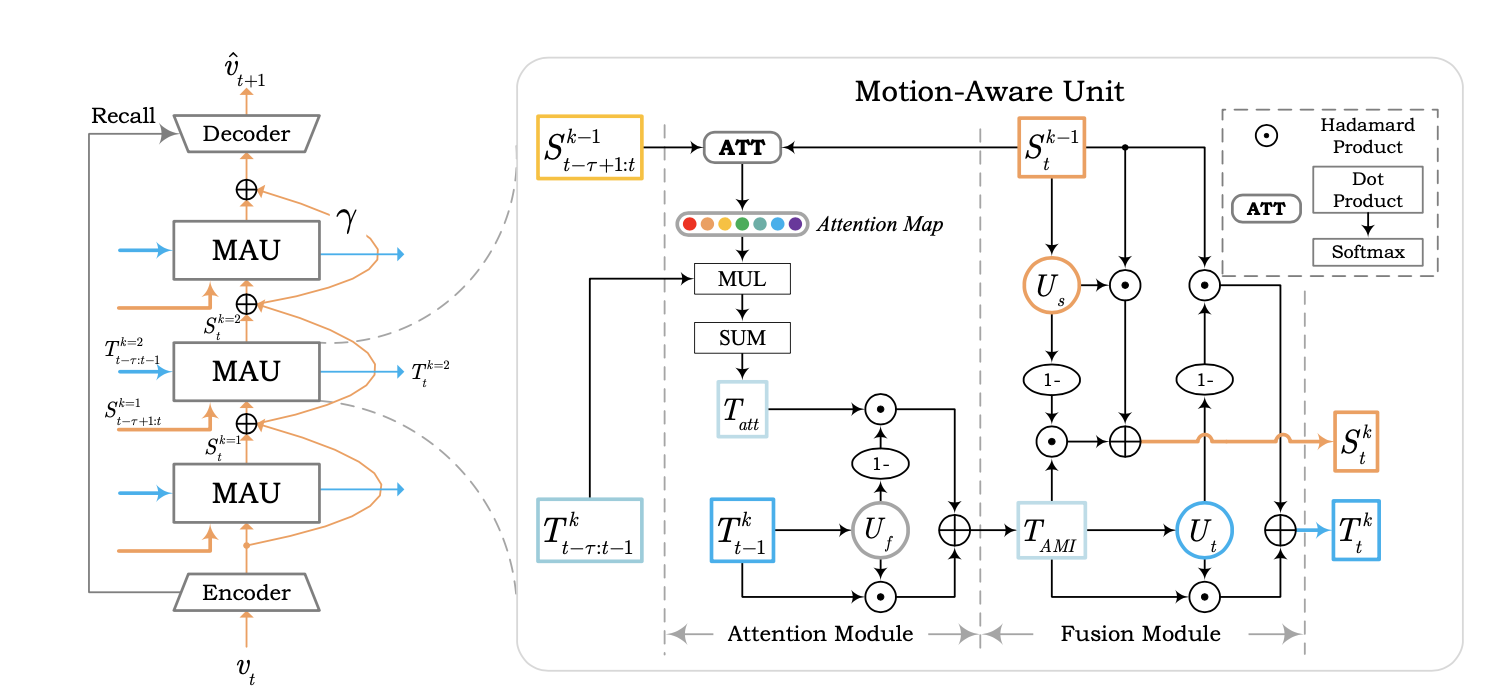
\includegraphics[width=\textwidth]{figures/mau.png}
            \caption{}
            \label{fig:exp1_mean_intensity_longitude_line}
          \end{figure}
          
          さらに、全球での評価と同様に、出力シークエンスの最後のタイムステップにおいて、動画予測モデルの出力から計算される経度ごとの平均輝度と、実際の観測画像での経度ごとの平均輝度をプロットした散布図を図\ref{fig:exp1_mean_intensity_longitude_scatter}に示す。
          
          \begin{figure}[htpb]
            \centering
            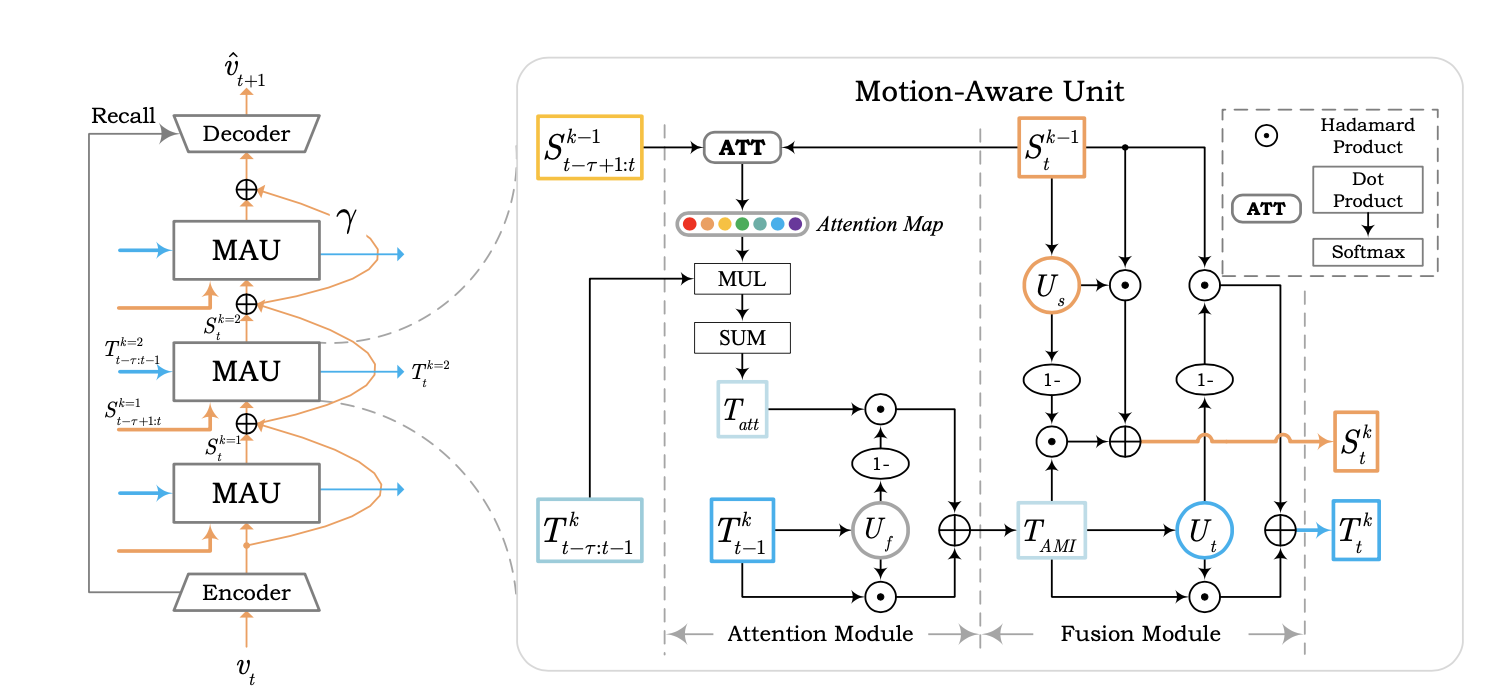
\includegraphics[width=\textwidth]{figures/mau.png}
            \caption{}
            \label{fig:exp1_mean_intensity_longitude_scatter}
          \end{figure}

        \subsubsection{単純差動回転モデルとの比較}
          全球での場合と同様に、経度ごとの比較でも単純差動回転モデルとの比較を行った。その時間推移を図\ref{fig:exp1_sdr_longitude_line}に示す。
          \begin{figure}[htbp]
            \centering
            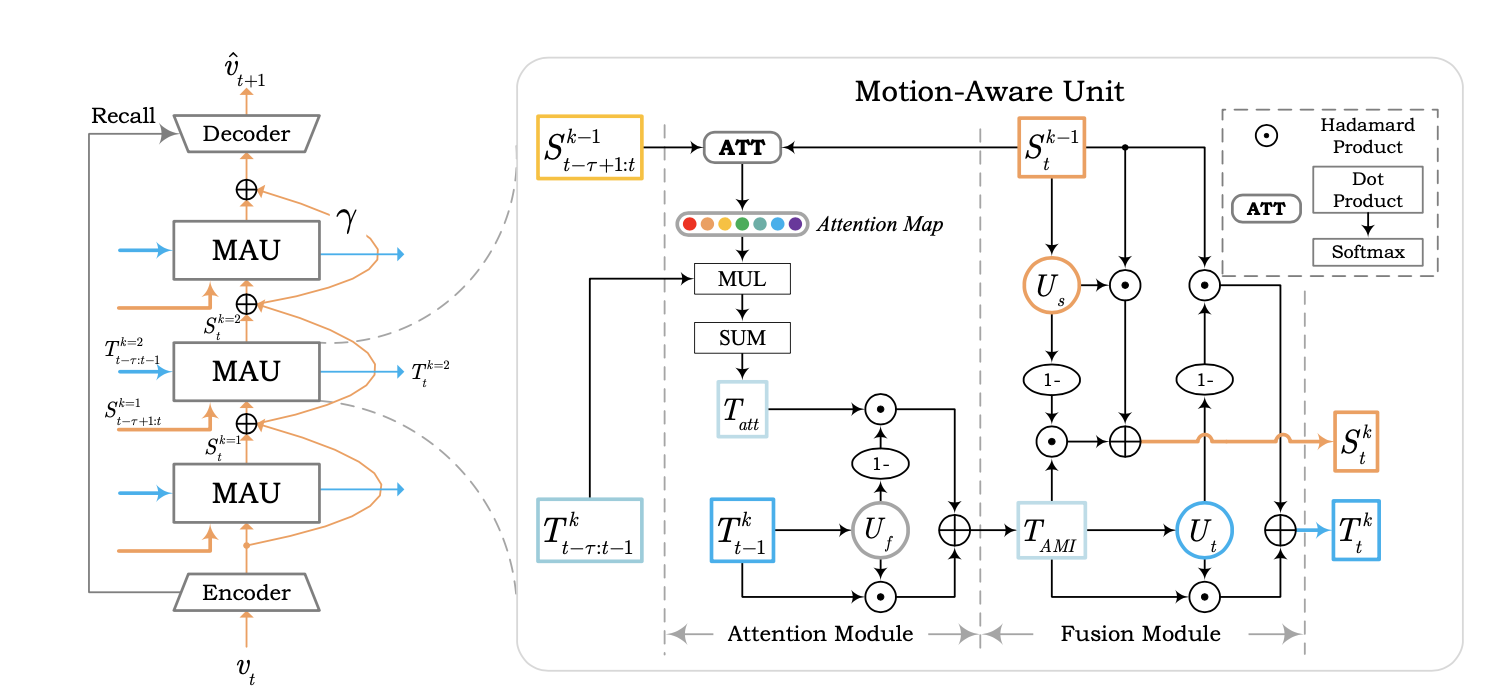
\includegraphics[width=\textwidth]{figures/mau.png}
            \caption{}
            \label{fig:exp1_sdr_longitude_line}
          \end{figure}
          
          また、出力シークエンスの最後のタイムステップにおける、経度ごとの単純差動回転モデルによるシミュレーションと、実際の観測画像との差異を観察し、動画予測モデルによる出力と比較した。
          その散布図を図\ref{fig:exp1_sdr_longitude_scatter}に示す。
          \begin{figure}[htbp]
            \centering
            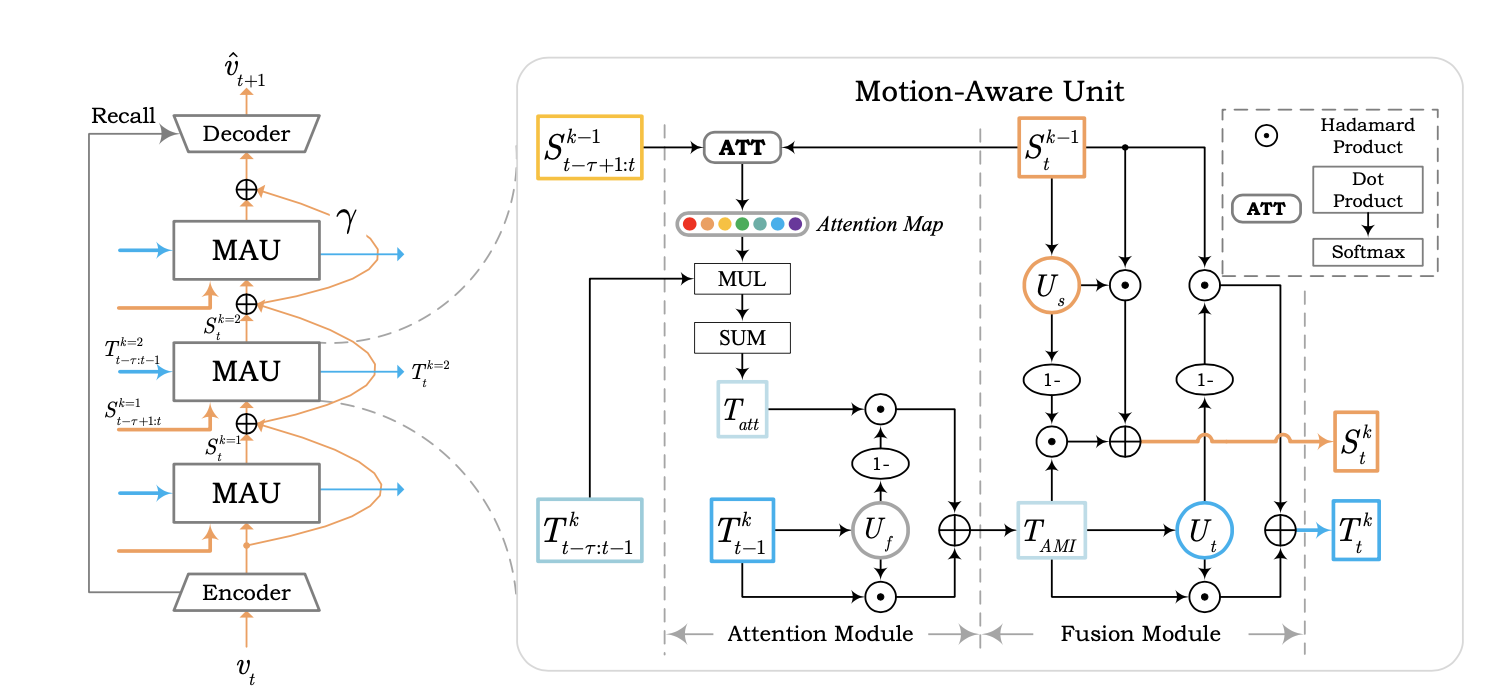
\includegraphics[width=\textwidth]{figures/mau.png}
            \caption{}
            \label{fig:exp1_sdr_longitude_scatter}
          \end{figure}
    
    \subsection{東側外縁部から出現する活動領域に対する視覚的評価}
      ここまでで、作成した動画予測モデルは、全球での平均輝度や、経度ごとの平均輝度といった定量的な評価において、実際の観測画像を正確に再現できていることを確認した。
      既存のシンプルなシミュレーションモデルとの比較でも、平均輝度の評価においては、動画予測モデルの優位性を確認できた。

      動画予測モデルのシミュレーションモデルに対するさらなる独自の特徴として、望遠鏡の視野に入っていない太陽の球面を生成することができる点が挙げられる。
      Sunpyによって提供される差動回転シミュレーションモデル\textit{physics.defferential\_rotation}は、入力された画像の全球面の各ピクセルに対して差動回転を適用することで画像を生成する。
      そのため、入力時点で望遠鏡の視野に入っていない太陽の球面を生成することができないので、より長い時間スパンでの予測を行うと、東の外縁部から徐々に予測できない領域が広がっていく。
      これに対して、動画予測モデルは、入力画像の全球面に対して特定の数理モデルを適用するのではなく、過去のデータや全体的な文脈を元に、視野に入っていなかった領域を含む未来の状態を生成する。
      
      ここでは、動画予測モデルが、そのような「入力画像の時点で全球面に見えていない領域」に対して予測能力を持つか検証を行うため、 生成された画像の東側外縁部から出現する活動領域に対する視覚的評価を行う。
      

  \section{考察}
